\clearpage

\section{Opaque with 1+1 Protection - Reference Network}
In this case study we focus on the opaque case with 1 + 1 protection for the reference network.

\subsection{Physical Network Topology}
\begin{tcolorbox}	
\begin{tabular}{p{2.75cm} p{0.2cm} p{10.5cm}} 	
\textbf{Student Name}  &:& Tiago Esteves    (October 03, 2017 - )\\
\end{tabular}
\end{tcolorbox}

In the figure below we ca see that our reference network is the same as in the subsection \ref{Reference_Network}.

\begin{figure}[h!]
\centering
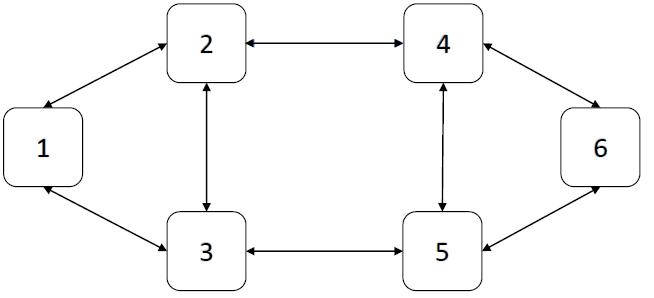
\includegraphics[width=\textwidth]{sdf/opaque/figures/RedeTeste}
\caption{Physical topology of the reference network.}
\end{figure}

The average length of the links, matrix of distances between the respective nodes and the ODU's matrices is the same as in the subsection \ref{Reference_Network_Topology} the same happens for the total network traffic for the two scenarios.\\

Finally for this case has to take into consideration the table \ref{table_ref_net} once again.


\subsection{Dimensioning using ILP}
\begin{tcolorbox}	
\begin{tabular}{p{2.75cm} p{0.2cm} p{10.5cm}} 	
\textbf{Student Name}  &:& Tiago Esteves    (October 03, 2017 - )\\
\end{tabular}
\end{tcolorbox}


In this section we will do the dimensioning of the network mentioned in the previous section to calculate the value of your CAPEX, for this we will use the ILP model describe in section \ref{ILP_Opaque_Protection} and we can get the best possible solution.
For this we will use MATLAB which is ideal for dealing with linear programming problems and can call the LPsolve through an external interface.
The network cost and all the formulas used in this section are the same used in subsection \ref{Net_Costs} as such if only we will mention one subsection where with the results obtained through the described model.\\


\textbf{Scenario 1: Reference Network Low Traffic} \label{Scenario1_opaque_p} \\

In this scenario we used the table \ref{table_ref_net}. In the table \ref{result_ILP1_p} we can see the values calculated through MatLab and using the values indicated in table \ref{table_cost_opaque} we can finally calculate the CAPEX value.
\begin{table}[h!]
\centering
\begin{tabular}{|| c | c||}
 \hline
 Number of optical channels & Value \\
 \hline\hline
 in the link (1,2) & 2 \\
 in the link (1,3) & 2 \\
 in the link (2,3) & 4 \\
 in the link (2,4) & 3 \\
 in the link (3,5) & 3 \\
 in the link (4,5) & 3 \\
 in the link (4,6) & 3 \\
 in the link (5,6) & 3 \\
 \hline
\end{tabular}
\caption{Table with results}
\label{result_ILP1_p}
\end{table}

Using equation \ref{linkCosts} : \\
$C_L$ = $($2 * 15 000 * 8$)$ + $($2 * 5 000 * 100 * 23$)$ + $($24 * 4 000$)$ \\
$C_L$ = \textbf{23 336 000\euro} \\

Using equation \ref{electricalCostOpaque} : \\
$C_{exc}$ = $($6 * 10 000$)$ + 1 000 * $($1 000 + $($2 * 23 * 100$)$ $)$ \\
$C_N$ = $C_{exc}$ = \textbf{5 660 000\euro} \\

$CAPEX$ = 23 336 000 + 5 660 000 = \textbf{28 996 000\euro}\\


\textbf{Scenario 2: Reference Network High Traffic} \label{Scenario2_opaque_p} \\

In this scenario we used again the table \ref{table_ref_net}. In the table \ref{result_ILP2_p} we can see the values calculated through MatLab and using the values indicated in table \ref{table_cost_opaque} we can finally calculate the CAPEX value.\\

\begin{table}[h!]
\centering
\begin{tabular}{|| c | c||}
 \hline
 Number of optical channels & Value \\
 \hline\hline
 in the link (1,2) & 12 \\
 in the link (1,3) & 12 \\
 in the link (2,3) & 33 \\
 in the link (2,4) & 28 \\
 in the link (3,5) & 28 \\
 in the link (4,5) & 26 \\
 in the link (4,6) & 30 \\
 in the link (5,6) & 30 \\
 \hline
\end{tabular}
\caption{Table with results}
\label{result_ILP2_p}
\end{table}


Using equation \ref{linkCosts} : \\
$C_L$ = $($2 * 15 000 * 8$)$ + $($2 * 5 000 * 100 * 199$)$ + $($24 * 4 000$)$ \\
$C_L$ = \textbf{199 336 000\euro} \\

Using equation \ref{electricalCostOpaque} : \\
$C_{exc}$ = $($6 * 10 000$)$ + 1 000 * $($10 000 + $($2 * 199 * 100$)$ $)$ \\
$C_N$ = $C_{exc}$ = \textbf{49 860 000\euro} \\

$CAPEX$ = 199 336 000 + 49 860 000 = \textbf{249 196 000\euro}\\

\subsection{Dimensioning using Heuristics}

\subsubsection{Heuristics Results}

\subsection{Comparative Analysis}

